\chapter{Многомодовые когерентные состояния и их интерференция}  \label{ch:ch4}
\section{Квантовое описание когерентного состояния} \label{sec:ch4/sec1}


\pagebreak

%%%%%%%%%%%%%%%%%%%%%%%%%%%%%%%%%%%%%%%%%%%%%%%%%%%%%%%%%%%%%%%%%%%%%%%%%%%%%%%%%%%%%%%%%%%%%%%%%%%%%%%%%%%%%%%%%
\section{Когерентные состояния после прохождения светоделителя} \label{ch:ch4/sect2}

 \begin{figure}[ht]
  \centering
  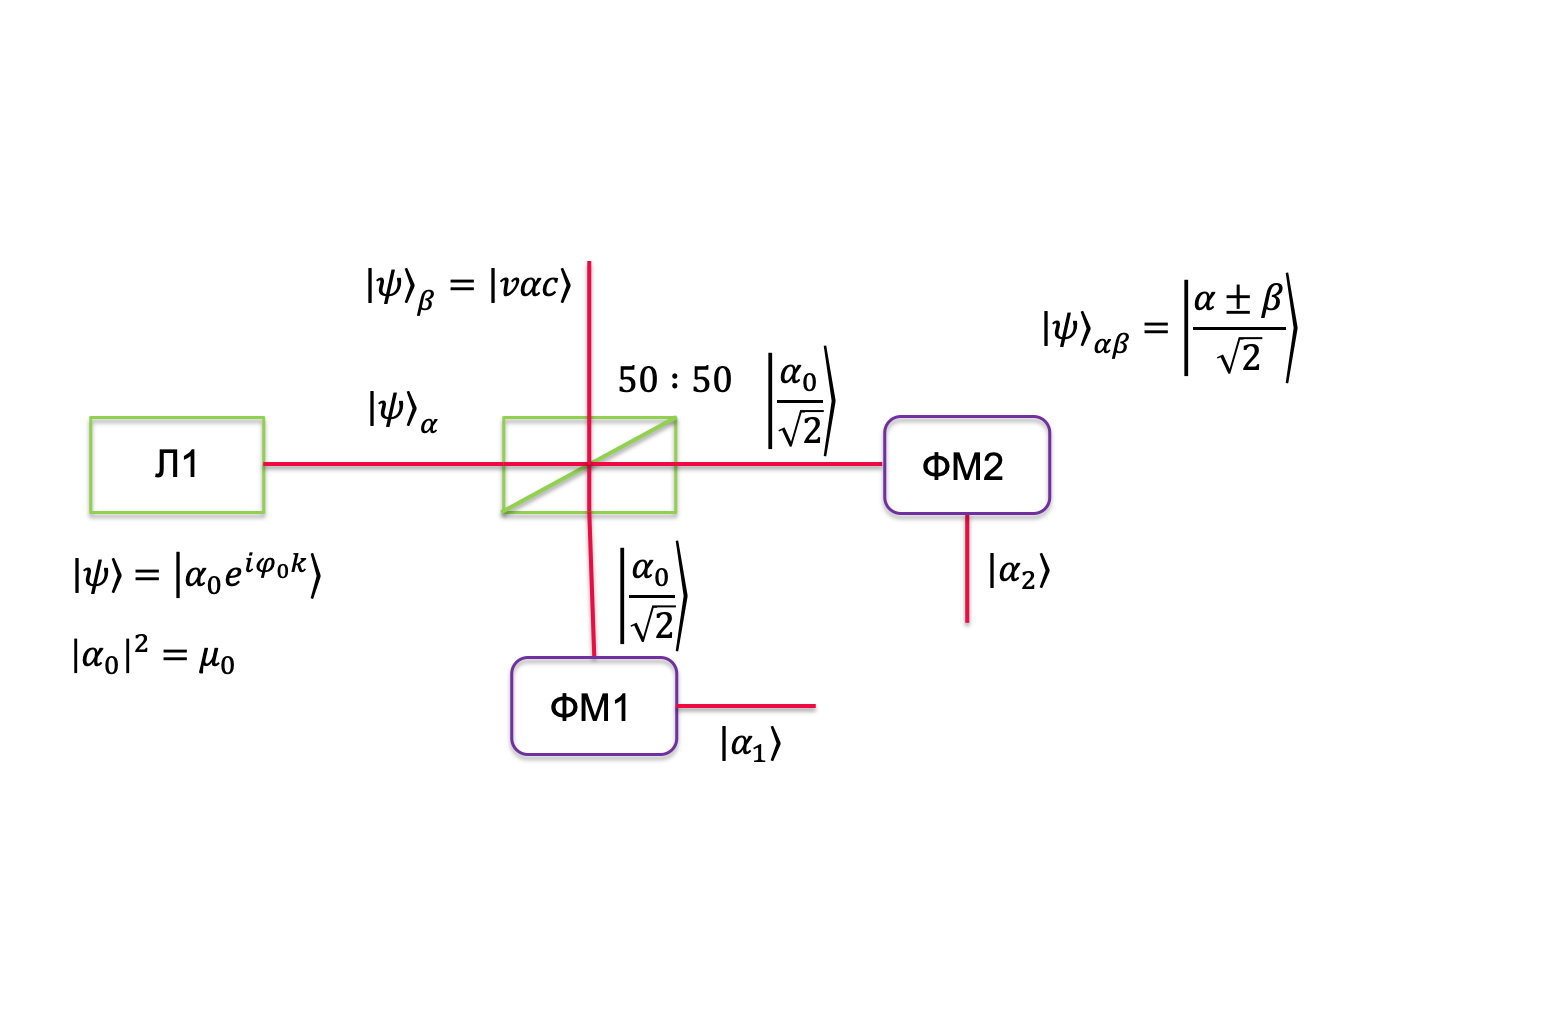
\includegraphics[scale=1]{Coherent_states_beamsplitting.png}
  \caption{Принципиальная схема наблюдения динамики когерентных состояний}
  \label{fig:Coherent_states_beamsplitting}
\end{figure}

\pagebreak

%%%%%%%%%%%%%%%%%%%%%%%%%%%%%%%%%%%%%%%%%%%%%%%%%%%%%%%%%%%%%%%%%%%%%%%%%%%%%%%%%%%%%%%%%%%%%%%%%%%%%%%%%%%%%%%%%
\section{Когерентные состояния после модуляции} \label{ch:ch4/sect3}

 \begin{figure}[ht]
  \centering
  \includegraphics[scale=0.5]{Modes_rus.pdf}
  \caption{Принципиальная схема генерации боковых частот}
  \label{fig:multimodes}
\end{figure}

\pagebreak

%%%%%%%%%%%%%%%%%%%%%%%%%%%%%%%%%%%%%%%%%%%%%%%%%%%%%%%%%%%%%%%%%%%%%%%%%%%%%%%%%%%%%%%%%%%%%%%%%%%%%%%%%%%%%%%%%
\section{Результат интерференции когерентных состояний после модуляции} \label{ch:ch4/sect4}

\begin{figure}[ht]
 \centering
  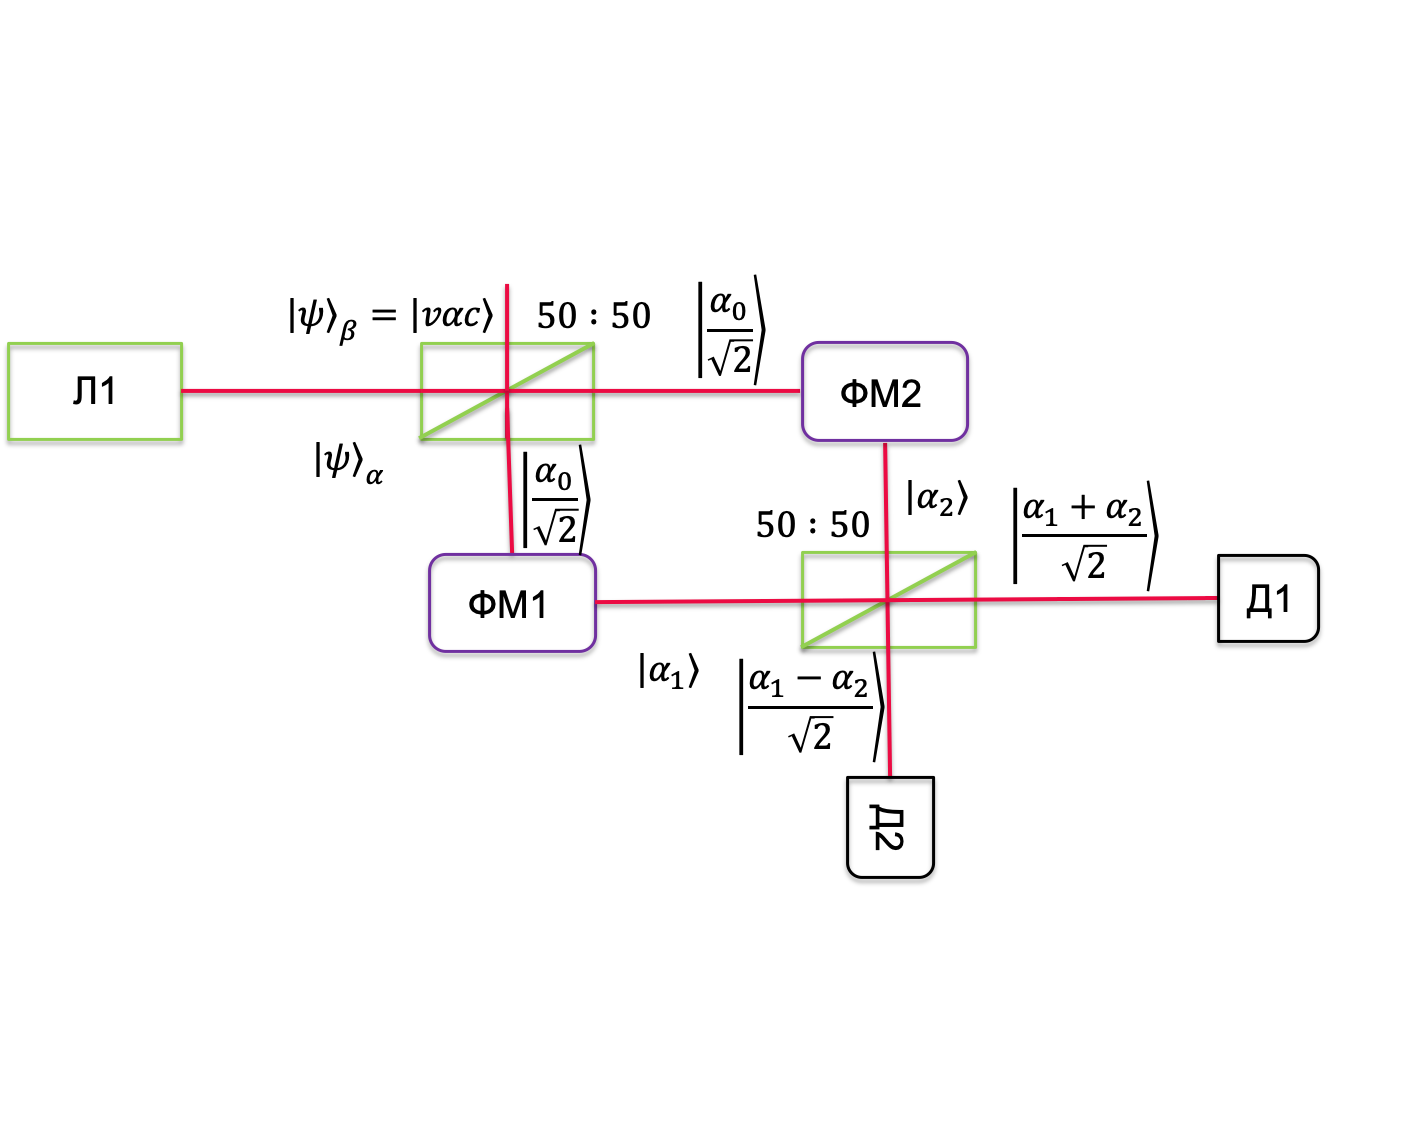
\includegraphics[scale=0.5]{Coherent_state_beamsplitting2.png}
  \caption{Принципиальная схема наблюдения динамики когерентных состояний}
  \label{fig:Coherent_states_beamsplitting2}
\end{figure}

\pagebreak

%%%%%%%%%%%%%%%%%%%%%%%%%%%%%%%%%%%%%%%%%%%%%%%%%%%%%%%%%%%%%%%%%%%%%%%%%%%%%%%%%%%%%%%%%%%%%%%%%%%%%%%%%%%%%%%%%
\section{Зависимость результата интерференции от разности фаз когерентных состояний} \label{ch:ch4/sect5}


\begin{figure}[ht]
 \centering
  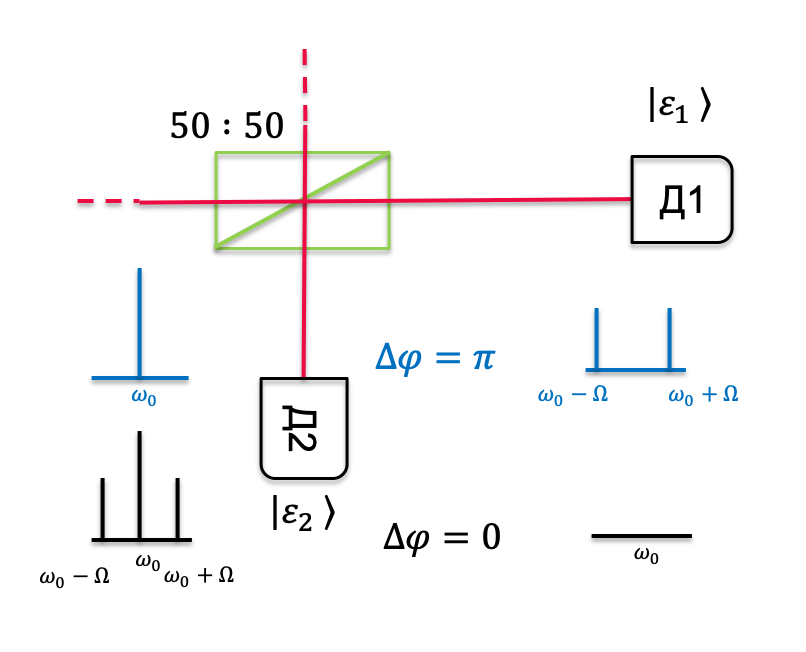
\includegraphics[scale=0.9]{Interference_result.png}
  \caption{Принципиальная схема наблюдения результата интерференции когерентных состояний}
  \label{fig:Interference_result}
\end{figure}

\pagebreak

%%%%%%%%%%%%%%%%%%%%%%%%%%%%%%%%%%%%%%%%%%%%%%%%%%%%%%%%%%%%%%%%%%%%%%%%%%%%%%%%%%%%%%%%%%%%%%%%%%%%%%%%%%%%%%%%%
\section{Протокол системы квантовой рассылки ключа, устойчивый к атакам на измерительное оборудование} \label{ch:ch4/sect6}

\begin{figure}[ht]
 \centering
  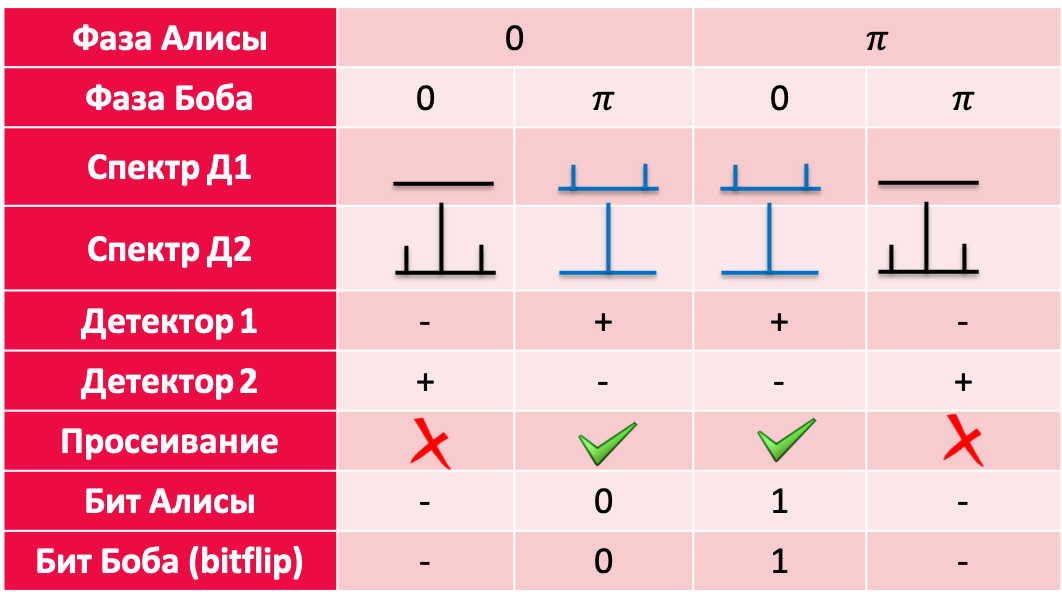
\includegraphics[scale=0.9]{Protocol.png}
  \caption{Протокол}
  \label{fig:Protocol}
\end{figure}


\pagebreak

%%%%%%%%%%%%%%%%%%%%%%%%%%%%%%%%%%%%%%%%%%%%%%%%%%%%%%%%%%%%%%%%%%%%%%%%%%%%%%%%%%%%%%%%%%%%%%%%%%%%%%%%%%%%%%%%%
\section{Выводы по главе} \label{ch:ch4/sect7}


Метод квантовой коммуникации на боковых частотах позволяет реализовывать протокол, устойчивый к контролю нелегитимным пользователем измерительного оборудования. 
 
\pagebreak

